\paragraph{Мейн}
В этой задаче исходный код функции отсутствует, программа не запускается, но есть информация, которую можно посмотреть в ghidra

\paragraph{Описание}
\begin{enumerate}
    \item Попытка запуска исполняемого файла без прав:
    \begin{verbatim}
    m@hp:~/Downloads/1$ ./task_2
    bash: ./task_2: Permission denied
    \end{verbatim}
    Вывод: нет прав на выполнение файла.

    \item Попытка запуска через \texttt{sudo}:
    \begin{verbatim}
    m@hp:~/Downloads/1$ sudo ./task_2
    [sudo] password for m:
    sudo: ./task_2: command not found
    \end{verbatim}
    Вывод: несмотря на \texttt{sudo}, команда не найдена.
    Файл не является исполняемым бинарником.
    Далее я посмотрел информацию о файле внутри ghidra, а также попробовал вывести все строчки с помощью команды \texttt{strings}
    \item Просмотр строк внутри файла через \texttt{strings}:
    \begin{verbatim}
    m@hp:~/Downloads/1$ strings task_2
    Linux
    Linux
    1Hello!
    1Bye-bye :(
    license=flag{baee49fd4f7009ff6e932463791f28e6}
    srcversion=FED0633F3F673540E886029
    depends=
    retpoline=Y
    name=task_7
    vermagic=6.2.0-34-generic SMP preempt mod_unload modversions
    __fentry__
    _printk
    __x86_return_thunk
    module_layout
    task_7
    GCC: (Ubuntu 11.4.0-1ubuntu1~22.04) 11.4.0
    GCC: (Ubuntu 11.4.0-1ubuntu1~22.04) 11.4.0
    .shstrtab
    .note.gnu.build-id
    .note.Linux
    .text
    .rodata.str1.1
    __mcount_loc
    .modinfo
    .return_sites
    .call_sites
    __versions
    __patchable_function_entries
    .exit.data
    .init.data
    .gnu.linkonce.this_module
    .bss
    .comment
    .note.GNU-stack
    \end{verbatim}

    \item Ключевой момент — найденная строка:
    \begin{verbatim}
    license=flag{baee49fd4f7009ff6e932463791f28e6}
    \end{verbatim}
\end{enumerate}

\vspace{0.5cm}

\noindent

\paragraph{Особенности}
\begin{itemize}
    \item Файл \texttt{task\_2} не является обычным исполняемым файлом, а представляет собой скомпилированный модуль ядра Linux.
    \item Запуск напрямую не работает, потому что модуль нужно загружать через \texttt{insmod} или \texttt{modprobe}, а не исполнять.
    \item Флаг хранится в строке с \texttt{license} внутри модуля.
    \item Флаг: flag\{baee49fd4f7009ff6e932463791f28e6\}
    \item В выводе присутсвует \("\)depends= \ldotsname=task\_7\ldots\("\), возможно этот файл содержит выводы для
    7го задания типа \("\)Hello!\("\) и \("\)Bye-bye :$($\("\).
    ФФлаг, найденный здесь, возможно, подойдет для решения 7й задачи.
\end{itemize}

\paragraph{Тестовые запуски} были в описании, поэтому прикреплю скриншот из гидры с полем лицензии и флага

\paragraph{}
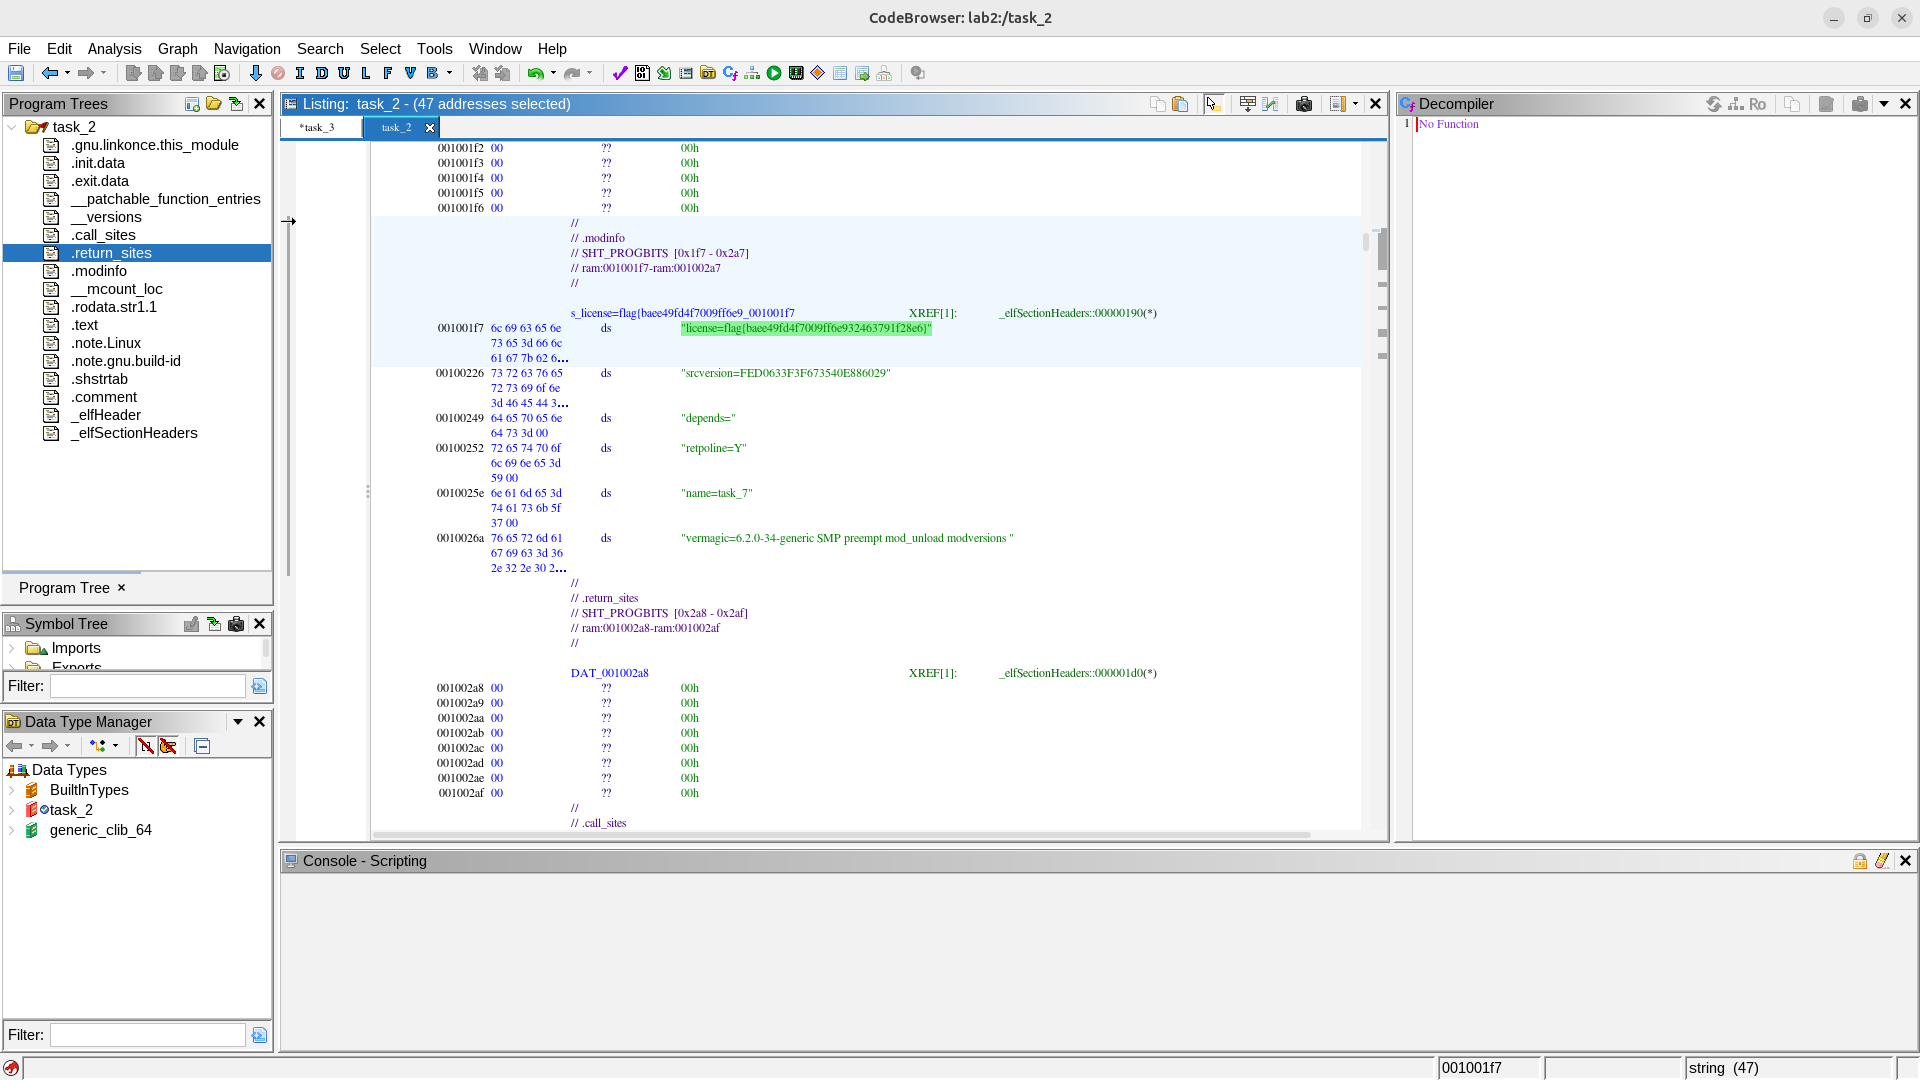
\includegraphics[width=1\linewidth]{static/solution_task_2}
